\section{線段樹}
    競賽上的版本。

    \subsection{用法與概念}

    線段樹除了可以用來快速解區間和問題,
    還可以用來執行許多與區間有關的操作。
    建構區間方式大致上如圖。

    \begin{figure}
        \centering
        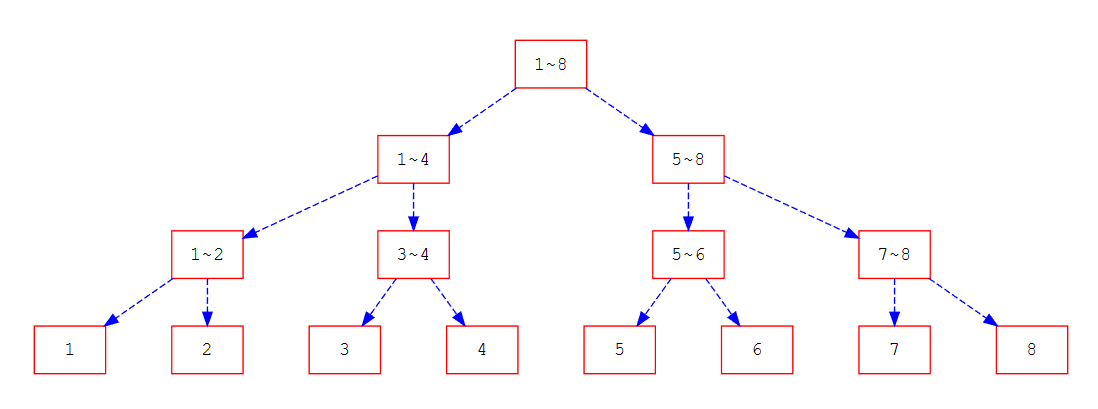
\includegraphics[width=\textwidth]{../Images/SEG.png}
    \end{figure}

    每個區間視情況放不同的數值,例如:最大/小,或是區間總和等。

    接著,每個區間就都可以分為$O(\log{(n)})$個區間,
    例如\verb|2-7|可以分為\verb|2, 3-4, 5-6, 7|。

    \begin{figure}
        \centering
        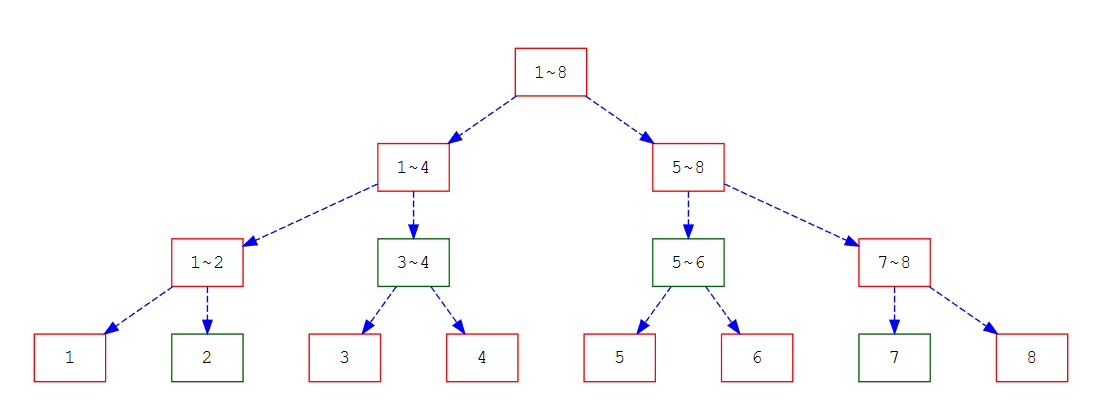
\includegraphics[width=\textwidth]{../Images/SEG2.png}
    \end{figure}

    查詢時皆以最大區間為出發點,
    如圖就會是從\verb|1-8|這個區間開始,如果要查詢的區間是\verb|2-7|。
    因為\verb|1-8|這個區間並沒有完全包含\verb|2-7|,
    因此需要往下遞迴,分成\verb|1-4|和\verb|5-8|再次查詢。

    接著,因為\verb|1-4|和\verb|5-8|仍然沒有完全被\verb|2-7|包含,
    因此要再次遞迴,這次是分解成\verb|1-2|,\verb|3-4|,\verb|5-6|以及\verb|7-8|。

    這次\verb|3-4|和\verb|5-6|都有被完全包含,
    因此可以直接回傳這個區間的值。而\verb|1-2|和\verb|7-8|還是沒有。
    所以這兩個區間還要再次向下查詢。

    查詢時最重要的是,若區間完全被包含就直接回傳,
    若完全沒被包含就不往那邊搜尋,
    否則再將區間分成兩塊向下遞迴。

    \subsection{實作}

    可以發現他是一顆二元樹,於是我們有兩種做法:指標型與陣列型。以下實作以區間總和為範例。

    \textbf{陣列型}

    \begin{tip}
        設根節點idx為1,在完滿二元樹中,左子樹就會是$idx \times 2$,右子樹就是$idx \times 2+1$。
    \end{tip}

\begin{lstlisting}[caption=陣列型線段樹]
#include<bits/stdc++.h>
using namespace std;

const int N=100010;

int a[N];
// 陣列seg的大小建議是N*4,否則你要先知道大於N的最小2^k值
// 131072 -> 262144 所以其實開 262200 就可以了
int seg[N*4];
int n,MXN=1;

// 不同於指標型的是:陣列型可以O(n)預建構
void build(int lb=1,int rb=MXN,int idx=1){
    //終止條件:區間長度為1
    if(lb==rb) return;
    
    // 設mid為區間中點,均分為左右區間
    // >>1相當於/2,但稍快
    int mid=lb+rb>>1;
    
    // idx*2   為左子樹
    // idx*2+1 為右子樹
    build(lb,mid,idx*2);
    build(mid+1,rb,idx*2+1);
    
    seg[idx]=seg[idx*2]+seg[idx*2+1];
}

void init(){
    // 為了讓他長度為2^k
    while(MXN<n) MXN<<=1;
    // 歸零
    for(int i=MXN+1;i<MXN*2;i++) seg[i]=0;
    // 以陣列的內容對其初始化
    for(int i=1;i<=n;++i) seg[MXN+i-1]=a[i];
    // 將所有節點都建構好
    build();
} 

void modify(int x,int k){
    // 此部分也與指標型不同,陣列可以直接依據座標修改
    x=x+MXN-1;
    seg[x]=k;
    
    // 向上更新節點
    while(x>1){
        x>>=1;
        seg[x]=seg[x*2]+seg[x*2+1];
    }
}

int query(int l,int r,int lb=1,int rb=MXN,int idx=1){
    // 終止條件:所在區間位於欲查詢區間之中
    if(l<=lb && rb<=r) return seg[idx];
    // 設mid為區間中點,均分為左右區間
    // >>1相當於/2,但稍快
    int mid=lb+rb>>1;

    int ret=0;
    if(l<=mid)   ret+=query(l,r, lb ,mid,idx*2);
    if(r>=mid+1) ret+=query(l,r,mid+1,rb,idx*2+1);
    
    return ret;
}

int main(){
    ios::sync_with_stdio(0);cin.tie(0);
    
    cin>>n;
    for(int i=1;i<=n;++i) cin>>a[i];
    // 一定要記得init()
    init();
}    
\end{lstlisting}

    \textbf{指標型}

\begin{lstlisting}[caption=指標型線段樹]
#include<bits/stdc++.h>
using namespace std;

int n;

struct node{
    // value
    int val;
    // 左右子樹的指標
    node *rch,*lch;
    // 建構式
    node(){
        val=0;
        rch=lch=nullptr;
    }
    // 帶有初始值的建構式
    node(int v){
        val=v;
        rch=lch=nullptr;
    }
    // 當左右子樹改變時,應重新計算父節點的值
    void pull(){
        // 歸零
        val=0;
        // 必須先有左右子樹才能拜訪
        // if(l) 相當於 if(l!=nullptr)
        if(lch) val+=lch->val;
        if(rch) val+=rch->val;
    }
    // 單點修改
    void modify(int p,int v,int lb=1,int rb=n){
        // 終止條件:區間長度為1
        if(lb==rb){
            val=v;
            return;
        }
        // 若左右子樹沒有結點則開一個新的
        if(!lch) lch=new node();
        if(!rch) rch=new node();
        // 設mid為區間中點,均分為左右區間
        // >>1相當於/2,但快很多
        int mid=lb+rb>>1;
        // 左邊走左,右邊走右
        if(p<=mid) lch->modify(p,v, lb ,mid);
        if(mid<p)  rch->modify(p,v,mid+1,rb);
        // 還記得子樹修改完要做什麼?
        pull();
    }

    int query(int l,int r,int lb=1,int rb=n){
        // 終止條件:所在區間位於欲查詢區間之中
        if(l<=lb && rb<=r){
            return val;
        }
        // 同modify
        int mid=lb+rb>>1;
        
        int ret=0;
        if(lch && l<=mid) ret+=lch->query(l,r, lb ,mid);
        if(rch && mid<r)  ret+=rch->query(l,r,mid+1,rb);
        // 為求保險
        pull();
        return ret;
    }
};

node *rt=new node();//root
\end{lstlisting}

    \subsection{範例與練習}
    \problem ZJe409 Segment Tree

    \textbf{題目敘述}

    你需要使用線段樹支援兩種操作。
    
    \begin{enumerate}
        \item 將 $A[x]$ 的值更新為 $y$
        \item 要查詢 $A[X]$-$A[Y]$ 之中最大值$maxA$及最小值$minA$的差
    \end{enumerate}

    \problem 戰術資料庫(110宜中資訊社校內賽pF)

    \textbf{題目敘述}

    要求能在一個陣列中做以下操作。

    \begin{enumerate}
        \item 搜尋區間和
        \item 搜尋區間最大和最小值
        \item 單點加減值
    \end{enumerate}

    \textbf{輸入說明}

    輸入第一行有一個數字 $n, q$ ,下一行有 $n$ 個數字,緊接著有 $q$ 筆操作,可能為以下五種。

    \begin{enumerate}
        \item 搜尋區間和 $find \; sum$ $(l)$ $(r)$
        \item 搜尋區間最大和最小值 $find$ $max/min (l)$ $(r)$
        \item 單點加減值 $plus/minus$ $(position)$ $(k)$
    \end{enumerate}

    相鄰數字間以空白隔開。
    $n, q \leq 100000 , a[i] \leq 100000$


    \textbf{輸出說明}

    對於每個搜尋指令做出回答。

    \textbf{範例測試}

    \begin{tabular}{|m{7cm}|m{7cm}|}
        \hline
        範例輸入 1 & 範例輸出 1 \\
        \hline
        \verb|7 10|          & \verb|5| \\
        \verb|1 2 3 4 5 6 7| & \verb|1| \\
        \verb|find max 2 5|  & \verb|31| \\
        \verb|find min 1 4|  & \verb|9| \\
        \verb|minus 3 1|     & \verb|6| \\
        \verb|plus 2 4|      & \\
        \verb|find sum 1 7| & \\
        \verb|plus 7 -3| & \\
        \verb|find sum 1 3| & \\
        \verb|minus 6 0| & \\
        \verb|plus 1 1| & \\
        \verb|find max 1 7| & \\
        \hline
    \end{tabular}